%---------------------------------------------------------------------------- 
%
%  $Description: General Research Plan Structure $
%
%  $Author: dloubach, with great contribution of rbonna $
%  $Release Date: December 20, 2016 $
%
%  O Projeto de Pesquisa deve demonstrar claramente os desafios científicos ou 
%  técnicos a serem superados pela pesquisa proposta, os meios e métodos para 
%  isso e a relevância dos resultados esperados para o avanço do conhecimento 
%  na área.
%  Máximo 20 páginas.
%
%  The research project shall clearly demonstrate the scientific or techinical
%  chalenges to be overcame by the proposed research, as well as the ways and
%  methods to achieve so and moreover the expected results relevance to advance
%  the area knowledgement.
%  20 pages maximum.
%---------------------------------------------------------------------------- 
\documentclass[12pt,a4paper]{article}
\usepackage{general-settings}
\usepackage{review-settings}

% title definitions
\newcommand{\titulo}{O Excelente Título para a sua Excelente Pesquisa}
\newcommand{\tituloI}{The Great Title of your Great Research}

% research level definitions
\newcommand{\subtitulo}{Projeto de Pesquisa de [Graduação|Mestrado|Doutorado]}
\newcommand{\aluno}{Seu Nome Vai Aqui}
\newcommand{\orientador}{Denis S. Loubach}

\newcommand{\ck}{\rule{8pt}{8pt}}

\linespread{1.3}

\begin{document}
\begin{titlepage}
	\begin{center}
		
		% Upper part of the page
		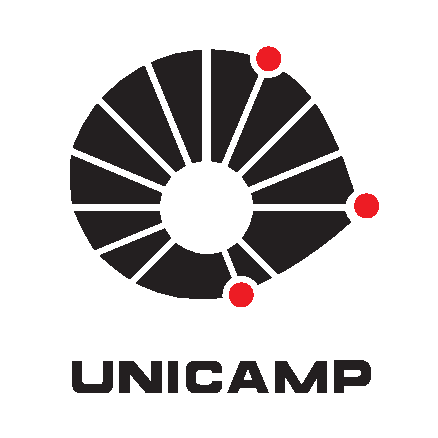
\includegraphics[scale=0.5]{unicamp.eps}\\[1cm]
		\textsc{\LARGE Universidade Estadual de Campinas}\\[1cm]
		
		\hrule
		\vspace{0.5cm}
		\textsc{\Large \titulo}\\[0.25cm]
      \textit{\tituloI}\\[0.5cm]
		{\large \subtitulo}\\[0.5cm]
		\hrule
		\vspace{2cm}
		% Author and supervisor
		\begin{minipage}{0.4\textwidth}
		    \begin{flushleft} \large
			    \emph{Aluno:}\\
			    \aluno
			 \end{flushleft}
	    \end{minipage}
	    \begin{minipage}{0.4\textwidth}
		    \begin{flushright} \large
			    \emph{Orientador:} \\
			    Prof. Dr. \orientador
		    \end{flushright}
		\end{minipage}
		\vfill
		% Data
		{\large \today}
	\end{center}
\end{titlepage}
    
\tableofcontents

\newpage

\section*{Resumo}
\label{sec:resumo}
Aqui vai o resumo do seu trabalho...\\%

\textbf{Palavras chave --} palavra-chave$_1$; ...; palavra-chave$_n$.


\newpage
\section*{\textit{Abstract}}
\label{sec:abstract}
\textit{
  Your abstract goes here.
}\\%

\textit{\textbf{Keywords --} keyword$_1$, ..., keyword$_n$.}


\newpage
\section{Introdução}
\label{sec:introducao}
Aqui vai a introdução do seu trabalho, contextualizando o leitor no assunto principal da sua pesquisa.

Exemplo de figura \ref{fig:perf_flex}:

\begin{figure}[ht]
	\centering
	\tikzset{my node/.style={circle, inner color=#1!20, outer color=#1!50,
	  draw=#1!75, text=black}}
	\begin{tikzpicture}
	  \node[my node = red] at (1,5) {GPPs};
	  \node[my node = blue] at (9,1) {ASICs};
	  \node[my node = purple] (SA) at (5.5,3.5) {FPGAs};
		\draw[thick,-latex] (0,0) -- (10,0)
			node[pos=1,below left]{performance};
	  \draw[thick,-latex] (0,0) -- (0,6)
			node[pos=1,above left,rotate = 90]{flexibilidade};
		\draw[color=gray,double,thick,-latex'] (SA)++(40:1) -- ++(40:1);
	\end{tikzpicture}
	\caption{Performance vs. flexibilidade em GPPs, ASICs e FPGAs.
	  Adaptado de \cite{Bobda2007a}.}
	\label{fig:perf_flex}
\end{figure}


\section{Trabalhos Relacionados}
\label{sec:trabalhos-relacionados}
Esta seção deve apresentar, de forma breve, os principais trabalhos relacionados aos conceitos fundamentais da sua pesquisa.

Exemplo:\\%
O trabalho \cite{Loubach2016a} introduz um \textit{design} de reconfiguração em tempo de execução para sistemas embarcados reconfiguráveis visando sistemas aviônicos. Leva-se em consideração principalmente a performance e o consumo de energia para reconfiguração parcial e total. Baseado nos resultados obtidos para consumo de energia, tempo de reconfiguração e tamanho dos \textit{bitstreams} (bits de configuração de FPGAs), pode-se considerar que sistemas embarcados reconfiguráveis em tempo real são viáveis para serem utilizados em sistemas aviônicos de gerações futuras.

Busque dar uma visão ampla de trabalhos básicos fundamentais e também trabalhos mais recentes.


\section{Objetivo}
\label{sec:objetivo}
O objetivo desse trabalho de pesquisa consiste em ``o que vc vai fazer de pesquisa'', visando ``qual o benefício principal esperado'' .


\section{Escopo da Pesquisa}
\label{sec:escopo-da-pesquisa}
O escopo deste trabalho de pesquisa concentra-se nos seguintes tópicos principais:

\begin{itemize}
\item Estudar ``isso'';
\item Estudar ``aquilo'';
\item Definição de ``modelo/projeto/desing/.../o que vc estiver fazendo de principal''; e
\item Testes, verificação e validação da ``proposta'' utilizando um estudo de caso.
\end{itemize}


\section{Plano de Trabalho e Cronograma}
\label{sec:plano-trabalho-cronograma}
Deve se apresentar aqui as principais atividades desse plano de trabalho, bem como o cronograma proposto para realização destas atividades.

\begin{enumerate}[A.]
  \item Disciplinas obrigatórias;
  \item Revisão bibliográfica;  
  \item Estudo da ``técnica x, teorema y, modelos z'';  
  \item Estudo e testes básicos das plataformas de hardware;  
  \item Elaboração de uma proposta de ``core da sua pesquia'';
  \item Elaboração de experimentos práticos de hardware;  
  \item Testes e verificação do modelo proposto; e    
  \item Validação e refinamentos do modelo proposto.   
\end{enumerate}

\begin{table}[ht]
  \centering
  \caption{Exemplo de cronograma de atividades dividido em trimestres.
    \label{tab:cronograma}}
  \begin{tabular}{|c||c|c|c|c||c|c|c|c||c|c|c|c||c|c|c|c|}
    \hline
    & \multicolumn{4}{|c||}{2016 - 2017}
    & \multicolumn{4}{|c||}{2017 - 2018}
    & \multicolumn{4}{|c||}{2018 - 2019}
    & \multicolumn{4}{|c|}{2019 - 2020} \\ \hline \hline
    Trimestre & 3 & 4 & 1 & 2 & 3 & 4 & 1 & 2 & 3 & 4 & 1 & 2 &
      3 & 4 & 1 & 2 \\ \hline \hline
    A & x & x & \ck & \ck & & & & & & & & & & & & \\ \hline
    B & x & x & \ck &  & & & & & & & & & & & & \\ \hline
    C & & & \ck & \ck & & & & & & & & & & & & \\ \hline
    D & & & \ck & \ck & \ck & & & & & & & & & & & \\ \hline
    E & & & & & \ck & \ck & \ck & \ck & & & & & & & & \\ \hline
    F & & & & & & & & \ck & \ck & \ck & & & & & & \\ \hline
	  G & & & & & & & & & & \ck & \ck & \ck & & & & \\ \hline
	  H & & & & & & & & & & & & \ck & \ck & \ck & & \\ \hline
	  Local & \multicolumn{4}{|c||}{Brasil}
    & \multicolumn{4}{|c||}{Outro País?}
    & \multicolumn{4}{|c||}{Brasil}
    & \multicolumn{4}{|c|}{Brasil} \\ \hline
\end{tabular}
\end{table}

Legenda: \ck~ a ser realizado; x  concluído.


\section{Materiais e Métodos}
\label{sec:materiais-metodos}
Que materiais (placas de hardware, kits de desenvolvimento, itens de medição) são necessários para desenvolver sua pesquisa?

Quais os métodos que vc pretente utilizar para desenvolver sua pesquisa? Colocar este tipo de informação nesta seção.

\section{Forma de Análise de Resultados}
\label{sec:analise-resultados}
Como verificar/analisar se o que vc produziu está correto? \textit{Benchmark} disponível na literatura, estudos comparativos, reprodução de pesquisas? Como garantir a corretude dos resultados. Como verificar quão bom está o seu trabalho em relação ao que já existe atualmente?


\section{Estágio de Pesquisa no Exterior}
\label{sec:pesquisa-exterior}
Eventual estágio no exterior dizendo onde, qual o professor supervisor e as devidas justificativas para posterior solicitação formal do estágio de pesquisa no exterior.


% referências
\bibliographystyle{ieeetr}
\bibliography{refs/references}

% todo list
\listoftodos

\end{document}